\documentclass[twoside]{book}

% Packages required by doxygen
\usepackage{fixltx2e}
\usepackage{calc}
\usepackage{doxygen}
\usepackage[export]{adjustbox} % also loads graphicx
\usepackage{graphicx}
\usepackage[utf8]{inputenc}
\usepackage{makeidx}
\usepackage{multicol}
\usepackage{multirow}
\PassOptionsToPackage{warn}{textcomp}
\usepackage{textcomp}
\usepackage[nointegrals]{wasysym}
\usepackage[table]{xcolor}

% Font selection
\usepackage[T1]{fontenc}
\usepackage[scaled=.90]{helvet}
\usepackage{courier}
\usepackage{amssymb}
\usepackage{sectsty}
\renewcommand{\familydefault}{\sfdefault}
\allsectionsfont{%
  \fontseries{bc}\selectfont%
  \color{darkgray}%
}
\renewcommand{\DoxyLabelFont}{%
  \fontseries{bc}\selectfont%
  \color{darkgray}%
}
\newcommand{\+}{\discretionary{\mbox{\scriptsize$\hookleftarrow$}}{}{}}

% Page & text layout
\usepackage{geometry}
\geometry{%
  a4paper,%
  top=2.5cm,%
  bottom=2.5cm,%
  left=2.5cm,%
  right=2.5cm%
}
\tolerance=750
\hfuzz=15pt
\hbadness=750
\setlength{\emergencystretch}{15pt}
\setlength{\parindent}{0cm}
\setlength{\parskip}{3ex plus 2ex minus 2ex}
\makeatletter
\renewcommand{\paragraph}{%
  \@startsection{paragraph}{4}{0ex}{-1.0ex}{1.0ex}{%
    \normalfont\normalsize\bfseries\SS@parafont%
  }%
}
\renewcommand{\subparagraph}{%
  \@startsection{subparagraph}{5}{0ex}{-1.0ex}{1.0ex}{%
    \normalfont\normalsize\bfseries\SS@subparafont%
  }%
}
\makeatother

% Headers & footers
\usepackage{fancyhdr}
\pagestyle{fancyplain}
\fancyhead[LE]{\fancyplain{}{\bfseries\thepage}}
\fancyhead[CE]{\fancyplain{}{}}
\fancyhead[RE]{\fancyplain{}{\bfseries\leftmark}}
\fancyhead[LO]{\fancyplain{}{\bfseries\rightmark}}
\fancyhead[CO]{\fancyplain{}{}}
\fancyhead[RO]{\fancyplain{}{\bfseries\thepage}}
\fancyfoot[LE]{\fancyplain{}{}}
\fancyfoot[CE]{\fancyplain{}{}}
\fancyfoot[RE]{\fancyplain{}{\bfseries\scriptsize Generated by Doxygen }}
\fancyfoot[LO]{\fancyplain{}{\bfseries\scriptsize Generated by Doxygen }}
\fancyfoot[CO]{\fancyplain{}{}}
\fancyfoot[RO]{\fancyplain{}{}}
\renewcommand{\footrulewidth}{0.4pt}
\renewcommand{\chaptermark}[1]{%
  \markboth{#1}{}%
}
\renewcommand{\sectionmark}[1]{%
  \markright{\thesection\ #1}%
}

% Indices & bibliography
\usepackage{natbib}
\usepackage[titles]{tocloft}
\setcounter{tocdepth}{3}
\setcounter{secnumdepth}{5}
\makeindex

% Hyperlinks (required, but should be loaded last)
\usepackage{ifpdf}
\ifpdf
  \usepackage[pdftex,pagebackref=true]{hyperref}
\else
  \usepackage[ps2pdf,pagebackref=true]{hyperref}
\fi
\hypersetup{%
  colorlinks=true,%
  linkcolor=blue,%
  citecolor=blue,%
  unicode%
}

% Custom commands
\newcommand{\clearemptydoublepage}{%
  \newpage{\pagestyle{empty}\cleardoublepage}%
}

\usepackage{caption}
\captionsetup{labelsep=space,justification=centering,font={bf},singlelinecheck=off,skip=4pt,position=top}

%===== C O N T E N T S =====

\begin{document}

% Titlepage & ToC
\hypersetup{pageanchor=false,
             bookmarksnumbered=true,
             pdfencoding=unicode
            }
\pagenumbering{alph}
\begin{titlepage}
\vspace*{7cm}
\begin{center}%
{\Large My Project }\\
\vspace*{1cm}
{\large Generated by Doxygen 1.8.13}\\
\end{center}
\end{titlepage}
\clearemptydoublepage
\pagenumbering{roman}
\tableofcontents
\clearemptydoublepage
\pagenumbering{arabic}
\hypersetup{pageanchor=true}

%--- Begin generated contents ---
\chapter{Hierarchical Index}
\section{Class Hierarchy}
This inheritance list is sorted roughly, but not completely, alphabetically\+:\begin{DoxyCompactList}
\item \contentsline{section}{Client}{\pageref{classClient}}{}
\item \contentsline{section}{Game\+Mech}{\pageref{classGameMech}}{}
\item \contentsline{section}{Grid}{\pageref{classGrid}}{}
\item \contentsline{section}{Gui}{\pageref{classGui}}{}
\item \contentsline{section}{Player}{\pageref{classPlayer}}{}
\begin{DoxyCompactList}
\item \contentsline{section}{Bot\+Ai}{\pageref{classBotAi}}{}
\item \contentsline{section}{User}{\pageref{classUser}}{}
\end{DoxyCompactList}
\item \contentsline{section}{Server}{\pageref{classServer}}{}
\item \contentsline{section}{Ship}{\pageref{classShip}}{}
\item \contentsline{section}{Square}{\pageref{classSquare}}{}
\end{DoxyCompactList}

\chapter{Class Index}
\section{Class List}
Here are the classes, structs, unions and interfaces with brief descriptions\+:\begin{DoxyCompactList}
\item\contentsline{section}{\hyperlink{classBotAi}{Bot\+Ai} }{\pageref{classBotAi}}{}
\item\contentsline{section}{\hyperlink{classClient}{Client} }{\pageref{classClient}}{}
\item\contentsline{section}{\hyperlink{classGameMech}{Game\+Mech} }{\pageref{classGameMech}}{}
\item\contentsline{section}{\hyperlink{classGrid}{Grid} }{\pageref{classGrid}}{}
\item\contentsline{section}{\hyperlink{classGui}{Gui} }{\pageref{classGui}}{}
\item\contentsline{section}{\hyperlink{classPlayer}{Player} }{\pageref{classPlayer}}{}
\item\contentsline{section}{\hyperlink{classServer}{Server} }{\pageref{classServer}}{}
\item\contentsline{section}{\hyperlink{classShip}{Ship} }{\pageref{classShip}}{}
\item\contentsline{section}{\hyperlink{classSquare}{Square} }{\pageref{classSquare}}{}
\item\contentsline{section}{\hyperlink{classUser}{User} }{\pageref{classUser}}{}
\end{DoxyCompactList}

\chapter{Class Documentation}
\hypertarget{classBotAi}{}\section{Bot\+Ai Class Reference}
\label{classBotAi}\index{Bot\+Ai@{Bot\+Ai}}


{\ttfamily \#include $<$Bot\+Ai.\+h$>$}



Inheritance diagram for Bot\+Ai\+:
\nopagebreak
\begin{figure}[H]
\begin{center}
\leavevmode
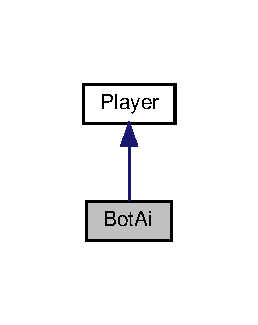
\includegraphics[width=124pt]{classBotAi__inherit__graph}
\end{center}
\end{figure}


Collaboration diagram for Bot\+Ai\+:
\nopagebreak
\begin{figure}[H]
\begin{center}
\leavevmode
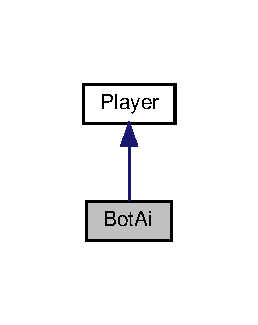
\includegraphics[width=124pt]{classBotAi__coll__graph}
\end{center}
\end{figure}
\subsection*{Public Member Functions}
\begin{DoxyCompactItemize}
\item 
\hyperlink{classBotAi_af1cef6cb4b7d04919265e073443e1fc9}{Bot\+Ai} (int p)
\item 
\hyperlink{classBotAi_aeb58b1fa5a7fcf2bd51a3242f21e8b09}{Bot\+Ai} ()
\item 
void \hyperlink{classBotAi_a26e701cc128abb1862c49e4cad249a12}{generate\+Ai\+Ships} ()
\item 
int $\ast$ \hyperlink{classBotAi_a27834ee25890a2c462fcd3d318ca976f}{drop\+Random\+Bomb} ()
\item 
int $\ast$ \hyperlink{classBotAi_a3ec71cf63ede0307d303cda7d003051b}{drop\+Bomb\+Ai} ()
\end{DoxyCompactItemize}


\subsection{Detailed Description}
This class inherits all \hyperlink{classPlayer}{Player} methods and is used to create a bot \begin{DoxyAuthor}{Author}
Adham Kassem 

Jonathon Henly 
\end{DoxyAuthor}


\subsection{Constructor \& Destructor Documentation}
\mbox{\Hypertarget{classBotAi_af1cef6cb4b7d04919265e073443e1fc9}\label{classBotAi_af1cef6cb4b7d04919265e073443e1fc9}} 
\index{Bot\+Ai@{Bot\+Ai}!Bot\+Ai@{Bot\+Ai}}
\index{Bot\+Ai@{Bot\+Ai}!Bot\+Ai@{Bot\+Ai}}
\subsubsection{\texorpdfstring{Bot\+Ai()}{BotAi()}\hspace{0.1cm}{\footnotesize\ttfamily [1/2]}}
{\footnotesize\ttfamily Bot\+Ai\+::\+Bot\+Ai (\begin{DoxyParamCaption}\item[{int}]{p }\end{DoxyParamCaption})\hspace{0.3cm}{\ttfamily [inline]}}

This is the constructor that instantiates a bot into the game \begin{DoxyAuthor}{Author}
Adham Kassem 

Jonathon Henly 
\end{DoxyAuthor}

\begin{DoxyParams}{Parameters}
{\em p} & int (player number) \\
\hline
\end{DoxyParams}
\begin{DoxyReturn}{Returns}
none 
\end{DoxyReturn}
\mbox{\Hypertarget{classBotAi_aeb58b1fa5a7fcf2bd51a3242f21e8b09}\label{classBotAi_aeb58b1fa5a7fcf2bd51a3242f21e8b09}} 
\index{Bot\+Ai@{Bot\+Ai}!Bot\+Ai@{Bot\+Ai}}
\index{Bot\+Ai@{Bot\+Ai}!Bot\+Ai@{Bot\+Ai}}
\subsubsection{\texorpdfstring{Bot\+Ai()}{BotAi()}\hspace{0.1cm}{\footnotesize\ttfamily [2/2]}}
{\footnotesize\ttfamily Bot\+Ai\+::\+Bot\+Ai (\begin{DoxyParamCaption}{ }\end{DoxyParamCaption})\hspace{0.3cm}{\ttfamily [inline]}}

This is the constructor that instantiates a bot into the game \begin{DoxyAuthor}{Author}
Adham Kassem 

Jonathon Henly 
\end{DoxyAuthor}

\begin{DoxyParams}{Parameters}
{\em none} & \\
\hline
\end{DoxyParams}
\begin{DoxyReturn}{Returns}
none 
\end{DoxyReturn}


\subsection{Member Function Documentation}
\mbox{\Hypertarget{classBotAi_a3ec71cf63ede0307d303cda7d003051b}\label{classBotAi_a3ec71cf63ede0307d303cda7d003051b}} 
\index{Bot\+Ai@{Bot\+Ai}!drop\+Bomb\+Ai@{drop\+Bomb\+Ai}}
\index{drop\+Bomb\+Ai@{drop\+Bomb\+Ai}!Bot\+Ai@{Bot\+Ai}}
\subsubsection{\texorpdfstring{drop\+Bomb\+Ai()}{dropBombAi()}}
{\footnotesize\ttfamily int$\ast$ Bot\+Ai\+::drop\+Bomb\+Ai (\begin{DoxyParamCaption}{ }\end{DoxyParamCaption})\hspace{0.3cm}{\ttfamily [inline]}}

This drops a bomb at random coordinates against the user. This is smarter and implements a hueristic to influence drop location. \begin{DoxyAuthor}{Author}
Adham Kassem 

Jonathon Henly 
\end{DoxyAuthor}

\begin{DoxyParams}{Parameters}
{\em none} & \\
\hline
\end{DoxyParams}
\begin{DoxyReturn}{Returns}
coordinates int$\ast$ 
\end{DoxyReturn}
\mbox{\Hypertarget{classBotAi_a27834ee25890a2c462fcd3d318ca976f}\label{classBotAi_a27834ee25890a2c462fcd3d318ca976f}} 
\index{Bot\+Ai@{Bot\+Ai}!drop\+Random\+Bomb@{drop\+Random\+Bomb}}
\index{drop\+Random\+Bomb@{drop\+Random\+Bomb}!Bot\+Ai@{Bot\+Ai}}
\subsubsection{\texorpdfstring{drop\+Random\+Bomb()}{dropRandomBomb()}}
{\footnotesize\ttfamily int$\ast$ Bot\+Ai\+::drop\+Random\+Bomb (\begin{DoxyParamCaption}{ }\end{DoxyParamCaption})\hspace{0.3cm}{\ttfamily [inline]}}

This drops a bomb at random coordinates against the user. \begin{DoxyAuthor}{Author}
Adham Kassem 

Jonathon Henly 
\end{DoxyAuthor}

\begin{DoxyParams}{Parameters}
{\em none} & \\
\hline
\end{DoxyParams}
\begin{DoxyReturn}{Returns}
coordinates int$\ast$ 
\end{DoxyReturn}
\mbox{\Hypertarget{classBotAi_a26e701cc128abb1862c49e4cad249a12}\label{classBotAi_a26e701cc128abb1862c49e4cad249a12}} 
\index{Bot\+Ai@{Bot\+Ai}!generate\+Ai\+Ships@{generate\+Ai\+Ships}}
\index{generate\+Ai\+Ships@{generate\+Ai\+Ships}!Bot\+Ai@{Bot\+Ai}}
\subsubsection{\texorpdfstring{generate\+Ai\+Ships()}{generateAiShips()}}
{\footnotesize\ttfamily void Bot\+Ai\+::generate\+Ai\+Ships (\begin{DoxyParamCaption}{ }\end{DoxyParamCaption})\hspace{0.3cm}{\ttfamily [inline]}}

This randomly generates the ships for the bot. \begin{DoxyAuthor}{Author}
Adham Kassem 

Jonathon Henly 
\end{DoxyAuthor}

\begin{DoxyParams}{Parameters}
{\em none} & \\
\hline
\end{DoxyParams}
\begin{DoxyReturn}{Returns}
none 
\end{DoxyReturn}


The documentation for this class was generated from the following file\+:\begin{DoxyCompactItemize}
\item 
include/Bot\+Ai.\+h\end{DoxyCompactItemize}

\hypertarget{classClient}{}\section{Client Class Reference}
\label{classClient}\index{Client@{Client}}


The documentation for this class was generated from the following file\+:\begin{DoxyCompactItemize}
\item 
include/Client.\+h\end{DoxyCompactItemize}

\hypertarget{classGameMech}{}\section{Game\+Mech Class Reference}
\label{classGameMech}\index{Game\+Mech@{Game\+Mech}}


{\ttfamily \#include $<$Game\+Mech.\+h$>$}

\subsection*{Public Member Functions}
\begin{DoxyCompactItemize}
\item 
\hyperlink{classGameMech_a73735ea1dac66c896fe3befb4425b1ee}{Game\+Mech} ()
\item 
void \hyperlink{classGameMech_acd8210b1f72b612ac0f1c3fad6d4a1da}{get\+Ships\+From\+User\+Console} ()
\item 
void \hyperlink{classGameMech_a2e6458b7b49afecdba3b1c2103d7875d}{start\+Pvp} ()
\item 
void \hyperlink{classGameMech_aceb6fd4797f93d9ffa9601a16b05eea6}{start\+Pv\+Bot} ()
\item 
void \hyperlink{classGameMech_a92543cf17b1dab64543d3d08c6ea621b}{get\+User\+Input} ()
\item 
\mbox{\Hypertarget{classGameMech_ae80d651eabb590b343ee548c68a1ac96}\label{classGameMech_ae80d651eabb590b343ee548c68a1ac96}} 
int $\ast$ {\bfseries get\+Turn\+Input} ()
\end{DoxyCompactItemize}


\subsection{Detailed Description}
This class implements the game mechanics \begin{DoxyAuthor}{Author}
Adham Kassem 

Jonathon Henly 
\end{DoxyAuthor}


\subsection{Constructor \& Destructor Documentation}
\mbox{\Hypertarget{classGameMech_a73735ea1dac66c896fe3befb4425b1ee}\label{classGameMech_a73735ea1dac66c896fe3befb4425b1ee}} 
\index{Game\+Mech@{Game\+Mech}!Game\+Mech@{Game\+Mech}}
\index{Game\+Mech@{Game\+Mech}!Game\+Mech@{Game\+Mech}}
\subsubsection{\texorpdfstring{Game\+Mech()}{GameMech()}}
{\footnotesize\ttfamily Game\+Mech\+::\+Game\+Mech (\begin{DoxyParamCaption}{ }\end{DoxyParamCaption})\hspace{0.3cm}{\ttfamily [inline]}}

Constructor for game mechanics. \begin{DoxyAuthor}{Author}
Adham Kassem 

Jonathon Henly 
\end{DoxyAuthor}

\begin{DoxyParams}{Parameters}
{\em none} & \\
\hline
\end{DoxyParams}
\begin{DoxyReturn}{Returns}
none 
\end{DoxyReturn}


\subsection{Member Function Documentation}
\mbox{\Hypertarget{classGameMech_acd8210b1f72b612ac0f1c3fad6d4a1da}\label{classGameMech_acd8210b1f72b612ac0f1c3fad6d4a1da}} 
\index{Game\+Mech@{Game\+Mech}!get\+Ships\+From\+User\+Console@{get\+Ships\+From\+User\+Console}}
\index{get\+Ships\+From\+User\+Console@{get\+Ships\+From\+User\+Console}!Game\+Mech@{Game\+Mech}}
\subsubsection{\texorpdfstring{get\+Ships\+From\+User\+Console()}{getShipsFromUserConsole()}}
{\footnotesize\ttfamily void Game\+Mech\+::get\+Ships\+From\+User\+Console (\begin{DoxyParamCaption}{ }\end{DoxyParamCaption})\hspace{0.3cm}{\ttfamily [inline]}}

This asks user for input in placing their ships on the \hyperlink{classGrid}{Grid}. The coordinates inputted correspond to the coordinates of the face of the ship. The size will be specified and the user will be able to choose the direction the ship faces.

\begin{DoxyAuthor}{Author}
Adham Kassem 

Jonathon Henly 
\end{DoxyAuthor}

\begin{DoxyParams}{Parameters}
{\em none} & \\
\hline
\end{DoxyParams}
\begin{DoxyReturn}{Returns}
none 
\end{DoxyReturn}
\mbox{\Hypertarget{classGameMech_a92543cf17b1dab64543d3d08c6ea621b}\label{classGameMech_a92543cf17b1dab64543d3d08c6ea621b}} 
\index{Game\+Mech@{Game\+Mech}!get\+User\+Input@{get\+User\+Input}}
\index{get\+User\+Input@{get\+User\+Input}!Game\+Mech@{Game\+Mech}}
\subsubsection{\texorpdfstring{get\+User\+Input()}{getUserInput()}}
{\footnotesize\ttfamily void Game\+Mech\+::get\+User\+Input (\begin{DoxyParamCaption}{ }\end{DoxyParamCaption})\hspace{0.3cm}{\ttfamily [inline]}}

This starts a \hyperlink{classPlayer}{Player} vs Bot game. All of the game mechanics and processing is done locally thru the client. \begin{DoxyAuthor}{Author}
Adham Kassem 

Jonathon Henly 
\end{DoxyAuthor}

\begin{DoxyParams}{Parameters}
{\em none} & \\
\hline
\end{DoxyParams}
\begin{DoxyReturn}{Returns}
none 
\end{DoxyReturn}
\mbox{\Hypertarget{classGameMech_aceb6fd4797f93d9ffa9601a16b05eea6}\label{classGameMech_aceb6fd4797f93d9ffa9601a16b05eea6}} 
\index{Game\+Mech@{Game\+Mech}!start\+Pv\+Bot@{start\+Pv\+Bot}}
\index{start\+Pv\+Bot@{start\+Pv\+Bot}!Game\+Mech@{Game\+Mech}}
\subsubsection{\texorpdfstring{start\+Pv\+Bot()}{startPvBot()}}
{\footnotesize\ttfamily void Game\+Mech\+::start\+Pv\+Bot (\begin{DoxyParamCaption}{ }\end{DoxyParamCaption})\hspace{0.3cm}{\ttfamily [inline]}}

This starts a \hyperlink{classPlayer}{Player} vs Bot game. All of the game mechanics and processing is done locally thru the client.

\begin{DoxyAuthor}{Author}
Adham Kassem 

Jonathon Henly 
\end{DoxyAuthor}

\begin{DoxyParams}{Parameters}
{\em none} & \\
\hline
\end{DoxyParams}
\begin{DoxyReturn}{Returns}
none 
\end{DoxyReturn}
\mbox{\Hypertarget{classGameMech_a2e6458b7b49afecdba3b1c2103d7875d}\label{classGameMech_a2e6458b7b49afecdba3b1c2103d7875d}} 
\index{Game\+Mech@{Game\+Mech}!start\+Pvp@{start\+Pvp}}
\index{start\+Pvp@{start\+Pvp}!Game\+Mech@{Game\+Mech}}
\subsubsection{\texorpdfstring{start\+Pvp()}{startPvp()}}
{\footnotesize\ttfamily void Game\+Mech\+::start\+Pvp (\begin{DoxyParamCaption}{ }\end{DoxyParamCaption})\hspace{0.3cm}{\ttfamily [inline]}}

This starts a \hyperlink{classPlayer}{Player} vs \hyperlink{classPlayer}{Player} game. This calls client functionality that connects to the server and performs pvp functionality. \begin{DoxyAuthor}{Author}
Adham Kassem 

Jonathon Henly 
\end{DoxyAuthor}

\begin{DoxyParams}{Parameters}
{\em none} & \\
\hline
\end{DoxyParams}
\begin{DoxyReturn}{Returns}
none 
\end{DoxyReturn}


The documentation for this class was generated from the following file\+:\begin{DoxyCompactItemize}
\item 
include/Game\+Mech.\+h\end{DoxyCompactItemize}

\hypertarget{classGrid}{}\section{Grid Class Reference}
\label{classGrid}\index{Grid@{Grid}}


{\ttfamily \#include $<$Grid.\+h$>$}

\subsection*{Public Member Functions}
\begin{DoxyCompactItemize}
\item 
\hyperlink{classGrid_a2d8f94be7fddec75f8a5fcd39cfcf3cb}{Grid} (int p)
\item 
\hyperlink{classGrid_a4ac9ff4f63552b4c61ff90fcb35ad66c}{Grid} ()
\item 
void \hyperlink{classGrid_a713d836d20af92af9f88849406267ea0}{add\+Ship} (int s, int d, int y, int x)
\item 
int \hyperlink{classGrid_aecf93fb530503819997f56c8e9dc282c}{get\+Square} (int y, int x)
\item 
void \hyperlink{classGrid_a8d0393b3b893d201b4afd9062487a59f}{hit} (int x, int y)
\item 
string \hyperlink{classGrid_ac379e67e40e0cebc8d37dfba4147dfb0}{drop\+Bomb} (int x, int y)
\item 
unsigned char $\ast$ \hyperlink{classGrid_aeb14a686f7219799a7796fc4f270f5d9}{get\+Grid\+Stream} ()
\item 
string \hyperlink{classGrid_adde29f8454547c9e81ce2b3c2e95bc43}{to\+String} ()
\item 
void \hyperlink{classGrid_afffe02cb1a0511678d6fb20ff3db1236}{add\+Hit} (int x, int y)
\end{DoxyCompactItemize}


\subsection{Detailed Description}
This class implements the grid and grid functionalities used in game \begin{DoxyAuthor}{Author}
Adham Kassem 

Jonathon Henly 
\end{DoxyAuthor}


\subsection{Constructor \& Destructor Documentation}
\mbox{\Hypertarget{classGrid_a2d8f94be7fddec75f8a5fcd39cfcf3cb}\label{classGrid_a2d8f94be7fddec75f8a5fcd39cfcf3cb}} 
\index{Grid@{Grid}!Grid@{Grid}}
\index{Grid@{Grid}!Grid@{Grid}}
\subsubsection{\texorpdfstring{Grid()}{Grid()}\hspace{0.1cm}{\footnotesize\ttfamily [1/2]}}
{\footnotesize\ttfamily Grid\+::\+Grid (\begin{DoxyParamCaption}\item[{int}]{p }\end{DoxyParamCaption})\hspace{0.3cm}{\ttfamily [inline]}}

\hyperlink{classGrid}{Grid} constructor that instantiates a players grid and add ships to the grid. \begin{DoxyAuthor}{Author}
Adham Kassem 

Jonathon Henly 
\end{DoxyAuthor}

\begin{DoxyParams}{Parameters}
{\em none} & \\
\hline
\end{DoxyParams}
\begin{DoxyReturn}{Returns}
player\+Num int 
\end{DoxyReturn}
\mbox{\Hypertarget{classGrid_a4ac9ff4f63552b4c61ff90fcb35ad66c}\label{classGrid_a4ac9ff4f63552b4c61ff90fcb35ad66c}} 
\index{Grid@{Grid}!Grid@{Grid}}
\index{Grid@{Grid}!Grid@{Grid}}
\subsubsection{\texorpdfstring{Grid()}{Grid()}\hspace{0.1cm}{\footnotesize\ttfamily [2/2]}}
{\footnotesize\ttfamily Grid\+::\+Grid (\begin{DoxyParamCaption}{ }\end{DoxyParamCaption})\hspace{0.3cm}{\ttfamily [inline]}}

\hyperlink{classGrid}{Grid} constructor that instantiates a players grid which adds ships to the grid. \begin{DoxyAuthor}{Author}
Adham Kassem 

Jonathon Henly 
\end{DoxyAuthor}

\begin{DoxyParams}{Parameters}
{\em none} & \\
\hline
\end{DoxyParams}
\begin{DoxyReturn}{Returns}
none 
\end{DoxyReturn}


\subsection{Member Function Documentation}
\mbox{\Hypertarget{classGrid_afffe02cb1a0511678d6fb20ff3db1236}\label{classGrid_afffe02cb1a0511678d6fb20ff3db1236}} 
\index{Grid@{Grid}!add\+Hit@{add\+Hit}}
\index{add\+Hit@{add\+Hit}!Grid@{Grid}}
\subsubsection{\texorpdfstring{add\+Hit()}{addHit()}}
{\footnotesize\ttfamily void Grid\+::add\+Hit (\begin{DoxyParamCaption}\item[{int}]{x,  }\item[{int}]{y }\end{DoxyParamCaption})\hspace{0.3cm}{\ttfamily [inline]}}

This method is meant for user objects that represent the opponent user locally. When the server informs client that the clients turn was a hit, this method will change the local state of the grid for proper local visualization \begin{DoxyAuthor}{Author}
Adham Kassem 

Jonathon Henly 
\end{DoxyAuthor}

\begin{DoxyParams}{Parameters}
{\em x} & int \\
\hline
{\em y} & int \\
\hline
\end{DoxyParams}
\begin{DoxyReturn}{Returns}
none 
\end{DoxyReturn}
\mbox{\Hypertarget{classGrid_a713d836d20af92af9f88849406267ea0}\label{classGrid_a713d836d20af92af9f88849406267ea0}} 
\index{Grid@{Grid}!add\+Ship@{add\+Ship}}
\index{add\+Ship@{add\+Ship}!Grid@{Grid}}
\subsubsection{\texorpdfstring{add\+Ship()}{addShip()}}
{\footnotesize\ttfamily void Grid\+::add\+Ship (\begin{DoxyParamCaption}\item[{int}]{s,  }\item[{int}]{d,  }\item[{int}]{y,  }\item[{int}]{x }\end{DoxyParamCaption})\hspace{0.3cm}{\ttfamily [inline]}}

Adds a ship to the grid \begin{DoxyAuthor}{Author}
Adham Kassem 

Jonathon Henly 
\end{DoxyAuthor}

\begin{DoxyParams}{Parameters}
{\em size} & int \\
\hline
{\em direction} & int \\
\hline
{\em y} & coordinate int \\
\hline
{\em x} & coordinate int \\
\hline
\end{DoxyParams}
\begin{DoxyReturn}{Returns}
none 
\end{DoxyReturn}
\mbox{\Hypertarget{classGrid_ac379e67e40e0cebc8d37dfba4147dfb0}\label{classGrid_ac379e67e40e0cebc8d37dfba4147dfb0}} 
\index{Grid@{Grid}!drop\+Bomb@{drop\+Bomb}}
\index{drop\+Bomb@{drop\+Bomb}!Grid@{Grid}}
\subsubsection{\texorpdfstring{drop\+Bomb()}{dropBomb()}}
{\footnotesize\ttfamily string Grid\+::drop\+Bomb (\begin{DoxyParamCaption}\item[{int}]{x,  }\item[{int}]{y }\end{DoxyParamCaption})\hspace{0.3cm}{\ttfamily [inline]}}

Drops a bomb on this grid \begin{DoxyAuthor}{Author}
Adham Kassem 

Jonathon Henly 
\end{DoxyAuthor}

\begin{DoxyParams}{Parameters}
{\em y} & coordinate int \\
\hline
{\em x} & coordinate int \\
\hline
\end{DoxyParams}
\begin{DoxyReturn}{Returns}
outcome string (returns a string representation of outcome of this move \char`\"{}hit\char`\"{} or \char`\"{}miss\char`\"{}) 
\end{DoxyReturn}
\mbox{\Hypertarget{classGrid_aeb14a686f7219799a7796fc4f270f5d9}\label{classGrid_aeb14a686f7219799a7796fc4f270f5d9}} 
\index{Grid@{Grid}!get\+Grid\+Stream@{get\+Grid\+Stream}}
\index{get\+Grid\+Stream@{get\+Grid\+Stream}!Grid@{Grid}}
\subsubsection{\texorpdfstring{get\+Grid\+Stream()}{getGridStream()}}
{\footnotesize\ttfamily unsigned char$\ast$ Grid\+::get\+Grid\+Stream (\begin{DoxyParamCaption}{ }\end{DoxyParamCaption})\hspace{0.3cm}{\ttfamily [inline]}}

Returns a flat stream of unsigned char values that defines the grid state \begin{DoxyAuthor}{Author}
Adham Kassem 

Jonathon Henly 
\end{DoxyAuthor}

\begin{DoxyParams}{Parameters}
{\em none} & \\
\hline
\end{DoxyParams}
\begin{DoxyReturn}{Returns}
stream unsigned char$\ast$ 
\end{DoxyReturn}
\mbox{\Hypertarget{classGrid_aecf93fb530503819997f56c8e9dc282c}\label{classGrid_aecf93fb530503819997f56c8e9dc282c}} 
\index{Grid@{Grid}!get\+Square@{get\+Square}}
\index{get\+Square@{get\+Square}!Grid@{Grid}}
\subsubsection{\texorpdfstring{get\+Square()}{getSquare()}}
{\footnotesize\ttfamily int Grid\+::get\+Square (\begin{DoxyParamCaption}\item[{int}]{y,  }\item[{int}]{x }\end{DoxyParamCaption})\hspace{0.3cm}{\ttfamily [inline]}}

gets the square value of a specified coordinate in the grid. \begin{DoxyAuthor}{Author}
Adham Kassem 

Jonathon Henly 
\end{DoxyAuthor}

\begin{DoxyParams}{Parameters}
{\em y} & coordinate int \\
\hline
{\em x} & coordinate int \\
\hline
\end{DoxyParams}
\begin{DoxyReturn}{Returns}
none 
\end{DoxyReturn}
\mbox{\Hypertarget{classGrid_a8d0393b3b893d201b4afd9062487a59f}\label{classGrid_a8d0393b3b893d201b4afd9062487a59f}} 
\index{Grid@{Grid}!hit@{hit}}
\index{hit@{hit}!Grid@{Grid}}
\subsubsection{\texorpdfstring{hit()}{hit()}}
{\footnotesize\ttfamily void Grid\+::hit (\begin{DoxyParamCaption}\item[{int}]{x,  }\item[{int}]{y }\end{DoxyParamCaption})\hspace{0.3cm}{\ttfamily [inline]}}

If a part of a ship is hit, this method sets the square value to hit aka 2. \begin{DoxyAuthor}{Author}
Adham Kassem 

Jonathon Henly 
\end{DoxyAuthor}

\begin{DoxyParams}{Parameters}
{\em y} & coordinate int \\
\hline
{\em x} & coordinate int \\
\hline
\end{DoxyParams}
\begin{DoxyReturn}{Returns}
none 
\end{DoxyReturn}
\mbox{\Hypertarget{classGrid_adde29f8454547c9e81ce2b3c2e95bc43}\label{classGrid_adde29f8454547c9e81ce2b3c2e95bc43}} 
\index{Grid@{Grid}!to\+String@{to\+String}}
\index{to\+String@{to\+String}!Grid@{Grid}}
\subsubsection{\texorpdfstring{to\+String()}{toString()}}
{\footnotesize\ttfamily string Grid\+::to\+String (\begin{DoxyParamCaption}{ }\end{DoxyParamCaption})\hspace{0.3cm}{\ttfamily [inline]}}

Drops a bomb on this grid \begin{DoxyAuthor}{Author}
Adham Kassem 

Jonathon Henly 
\end{DoxyAuthor}

\begin{DoxyParams}{Parameters}
{\em none} & \\
\hline
\end{DoxyParams}
\begin{DoxyReturn}{Returns}
string (returns a string representation of the grid for visualization) 
\end{DoxyReturn}


The documentation for this class was generated from the following file\+:\begin{DoxyCompactItemize}
\item 
include/Grid.\+h\end{DoxyCompactItemize}

\hypertarget{classGui}{}\section{Gui Class Reference}
\label{classGui}\index{Gui@{Gui}}


The documentation for this class was generated from the following file\+:\begin{DoxyCompactItemize}
\item 
include/Gui.\+h\end{DoxyCompactItemize}

\hypertarget{classPlayer}{}\section{Player Class Reference}
\label{classPlayer}\index{Player@{Player}}


{\ttfamily \#include $<$Player.\+h$>$}



Inheritance diagram for Player\+:
\nopagebreak
\begin{figure}[H]
\begin{center}
\leavevmode
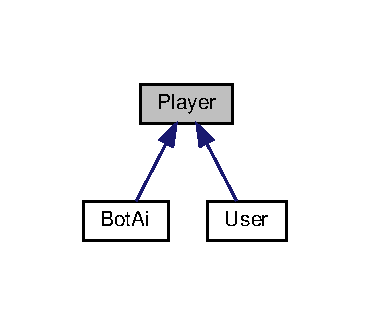
\includegraphics[width=178pt]{classPlayer__inherit__graph}
\end{center}
\end{figure}
\subsection*{Public Member Functions}
\begin{DoxyCompactItemize}
\item 
\mbox{\Hypertarget{classPlayer_a50cb6ccb69ac1d1613ff619fe686f062}\label{classPlayer_a50cb6ccb69ac1d1613ff619fe686f062}} 
{\bfseries Player} (int p)
\item 
\mbox{\Hypertarget{classPlayer_ad919a18f90221532a653a26f7233d3ab}\label{classPlayer_ad919a18f90221532a653a26f7233d3ab}} 
\hyperlink{classShip}{Ship} $\ast$ {\bfseries get\+Ships} ()
\item 
bool \hyperlink{classPlayer_a23d8eb40ae25ece11ecca4edfeb51738}{check\+If\+Valid} (int y, int x, int d, int s)
\item 
void \hyperlink{classPlayer_ab567a03f1c8fd3f61afc1dd9a54a1744}{set\+Ships} (\hyperlink{classShip}{Ship} $\ast$s)
\item 
\hyperlink{classGrid}{Grid} \hyperlink{classPlayer_a23a7fbedccc9bb48a0011878c0822912}{get\+Grid} ()
\item 
void \hyperlink{classPlayer_a8c60f8670782ecca840ce92fc3893e95}{set\+Grid} (\hyperlink{classGrid}{Grid} g1)
\item 
bool \hyperlink{classPlayer_af57244c7ed15bcae73e2eab5ecb81178}{did\+Lose} ()
\end{DoxyCompactItemize}


\subsection{Detailed Description}
This class implements \hyperlink{classPlayer}{Player} functionalities \begin{DoxyAuthor}{Author}
Adham Kassem 

Jonathon Henly 
\end{DoxyAuthor}


\subsection{Member Function Documentation}
\mbox{\Hypertarget{classPlayer_a23d8eb40ae25ece11ecca4edfeb51738}\label{classPlayer_a23d8eb40ae25ece11ecca4edfeb51738}} 
\index{Player@{Player}!check\+If\+Valid@{check\+If\+Valid}}
\index{check\+If\+Valid@{check\+If\+Valid}!Player@{Player}}
\subsubsection{\texorpdfstring{check\+If\+Valid()}{checkIfValid()}}
{\footnotesize\ttfamily bool Player\+::check\+If\+Valid (\begin{DoxyParamCaption}\item[{int}]{y,  }\item[{int}]{x,  }\item[{int}]{d,  }\item[{int}]{s }\end{DoxyParamCaption})\hspace{0.3cm}{\ttfamily [inline]}}

Checks to see if ship placement is valid \begin{DoxyAuthor}{Author}
Adham Kassem 

Jonathon Henly 
\end{DoxyAuthor}

\begin{DoxyParams}{Parameters}
{\em y} & coordinate int \\
\hline
{\em x} & coordinate int \\
\hline
{\em d} & direction int \\
\hline
{\em s} & size int \\
\hline
\end{DoxyParams}
\begin{DoxyReturn}{Returns}
is\+Valid boolean (returns whether or not the placement is valid) 
\end{DoxyReturn}
\mbox{\Hypertarget{classPlayer_af57244c7ed15bcae73e2eab5ecb81178}\label{classPlayer_af57244c7ed15bcae73e2eab5ecb81178}} 
\index{Player@{Player}!did\+Lose@{did\+Lose}}
\index{did\+Lose@{did\+Lose}!Player@{Player}}
\subsubsection{\texorpdfstring{did\+Lose()}{didLose()}}
{\footnotesize\ttfamily bool Player\+::did\+Lose (\begin{DoxyParamCaption}{ }\end{DoxyParamCaption})\hspace{0.3cm}{\ttfamily [inline]}}

Returns a boolean value on whether or not the player lost. \begin{DoxyAuthor}{Author}
Adham Kassem 

Jonathon Henly 
\end{DoxyAuthor}

\begin{DoxyParams}{Parameters}
{\em none} & \\
\hline
\end{DoxyParams}
\begin{DoxyReturn}{Returns}
did\+Lose boolean 
\end{DoxyReturn}
\mbox{\Hypertarget{classPlayer_a23a7fbedccc9bb48a0011878c0822912}\label{classPlayer_a23a7fbedccc9bb48a0011878c0822912}} 
\index{Player@{Player}!get\+Grid@{get\+Grid}}
\index{get\+Grid@{get\+Grid}!Player@{Player}}
\subsubsection{\texorpdfstring{get\+Grid()}{getGrid()}}
{\footnotesize\ttfamily \hyperlink{classGrid}{Grid} Player\+::get\+Grid (\begin{DoxyParamCaption}{ }\end{DoxyParamCaption})\hspace{0.3cm}{\ttfamily [inline]}}

getter for grid \begin{DoxyAuthor}{Author}
Adham Kassem 

Jonathon Henly 
\end{DoxyAuthor}

\begin{DoxyParams}{Parameters}
{\em none} & \\
\hline
\end{DoxyParams}
\begin{DoxyReturn}{Returns}
g \hyperlink{classGrid}{Grid} 
\end{DoxyReturn}
\mbox{\Hypertarget{classPlayer_a8c60f8670782ecca840ce92fc3893e95}\label{classPlayer_a8c60f8670782ecca840ce92fc3893e95}} 
\index{Player@{Player}!set\+Grid@{set\+Grid}}
\index{set\+Grid@{set\+Grid}!Player@{Player}}
\subsubsection{\texorpdfstring{set\+Grid()}{setGrid()}}
{\footnotesize\ttfamily void Player\+::set\+Grid (\begin{DoxyParamCaption}\item[{\hyperlink{classGrid}{Grid}}]{g1 }\end{DoxyParamCaption})\hspace{0.3cm}{\ttfamily [inline]}}

setter for grid \begin{DoxyAuthor}{Author}
Adham Kassem 

Jonathon Henly 
\end{DoxyAuthor}

\begin{DoxyParams}{Parameters}
{\em g1} & \hyperlink{classGrid}{Grid} \\
\hline
\end{DoxyParams}
\begin{DoxyReturn}{Returns}
none 
\end{DoxyReturn}
\mbox{\Hypertarget{classPlayer_ab567a03f1c8fd3f61afc1dd9a54a1744}\label{classPlayer_ab567a03f1c8fd3f61afc1dd9a54a1744}} 
\index{Player@{Player}!set\+Ships@{set\+Ships}}
\index{set\+Ships@{set\+Ships}!Player@{Player}}
\subsubsection{\texorpdfstring{set\+Ships()}{setShips()}}
{\footnotesize\ttfamily void Player\+::set\+Ships (\begin{DoxyParamCaption}\item[{\hyperlink{classShip}{Ship} $\ast$}]{s }\end{DoxyParamCaption})\hspace{0.3cm}{\ttfamily [inline]}}

setter for ships \begin{DoxyAuthor}{Author}
Adham Kassem 

Jonathon Henly 
\end{DoxyAuthor}

\begin{DoxyParams}{Parameters}
{\em s} & \hyperlink{classShip}{Ship} \\
\hline
\end{DoxyParams}
\begin{DoxyReturn}{Returns}
none 
\end{DoxyReturn}


The documentation for this class was generated from the following file\+:\begin{DoxyCompactItemize}
\item 
include/Player.\+h\end{DoxyCompactItemize}

\hypertarget{classServer}{}\section{Server Class Reference}
\label{classServer}\index{Server@{Server}}


The documentation for this class was generated from the following file\+:\begin{DoxyCompactItemize}
\item 
include/Server.\+h\end{DoxyCompactItemize}

\hypertarget{classShip}{}\section{Ship Class Reference}
\label{classShip}\index{Ship@{Ship}}


{\ttfamily \#include $<$Ship.\+h$>$}

\subsection*{Public Member Functions}
\begin{DoxyCompactItemize}
\item 
\hyperlink{classShip_ab7608fcfc4d27c678aacaf9bfd68a462}{Ship} ()
\item 
\hyperlink{classShip_a4d3829d2e927758bdb8ed7880e9403b4}{Ship} (int s, int d, int x1, int y1)
\item 
int \hyperlink{classShip_aafc09bad24dab9a7cb29e5c8f2b10226}{get\+Direction} ()
\item 
void \hyperlink{classShip_aa37f8f11f87ee3e17285816c5c6dc6f8}{set\+Direction} (int d)
\item 
int \hyperlink{classShip_aa741cc8f584a3fef5450d22cbde8a5f4}{get\+Size} ()
\item 
void \hyperlink{classShip_a764524af38d064e299e0ba90ae5f0a32}{set\+Size} (int s)
\item 
int \hyperlink{classShip_a846040dad9c03dec8d6bdfc24753f05b}{getX} ()
\item 
void \hyperlink{classShip_a060abd2e81215121f18112b88971161e}{setX} (int x1)
\item 
int \hyperlink{classShip_a0cde4e9b74fb71cbf61f79e0a1b74059}{getY} ()
\item 
void \hyperlink{classShip_a6637c65a27a5d08b151e1763ec67c4e6}{setY} (int y1)
\end{DoxyCompactItemize}


\subsection{Detailed Description}
This class stores \hyperlink{classShip}{Ship} info for each ship \begin{DoxyAuthor}{Author}
Adham Kassem 

Jonathon Henly 
\end{DoxyAuthor}


\subsection{Constructor \& Destructor Documentation}
\mbox{\Hypertarget{classShip_ab7608fcfc4d27c678aacaf9bfd68a462}\label{classShip_ab7608fcfc4d27c678aacaf9bfd68a462}} 
\index{Ship@{Ship}!Ship@{Ship}}
\index{Ship@{Ship}!Ship@{Ship}}
\subsubsection{\texorpdfstring{Ship()}{Ship()}\hspace{0.1cm}{\footnotesize\ttfamily [1/2]}}
{\footnotesize\ttfamily Ship\+::\+Ship (\begin{DoxyParamCaption}{ }\end{DoxyParamCaption})\hspace{0.3cm}{\ttfamily [inline]}}

Constructor for a \hyperlink{classShip}{Ship} object \begin{DoxyAuthor}{Author}
Adham Kassem 

Jonathon Henly 
\end{DoxyAuthor}
\mbox{\Hypertarget{classShip_a4d3829d2e927758bdb8ed7880e9403b4}\label{classShip_a4d3829d2e927758bdb8ed7880e9403b4}} 
\index{Ship@{Ship}!Ship@{Ship}}
\index{Ship@{Ship}!Ship@{Ship}}
\subsubsection{\texorpdfstring{Ship()}{Ship()}\hspace{0.1cm}{\footnotesize\ttfamily [2/2]}}
{\footnotesize\ttfamily Ship\+::\+Ship (\begin{DoxyParamCaption}\item[{int}]{s,  }\item[{int}]{d,  }\item[{int}]{x1,  }\item[{int}]{y1 }\end{DoxyParamCaption})\hspace{0.3cm}{\ttfamily [inline]}}

Constructor for a \hyperlink{classShip}{Ship} object \begin{DoxyAuthor}{Author}
Adham Kassem 

Jonathon Henly 
\end{DoxyAuthor}

\begin{DoxyParams}{Parameters}
{\em y} & coordinate int \\
\hline
{\em x} & coordinate int \\
\hline
{\em d} & direction int \\
\hline
{\em s} & size int \\
\hline
\end{DoxyParams}


\subsection{Member Function Documentation}
\mbox{\Hypertarget{classShip_aafc09bad24dab9a7cb29e5c8f2b10226}\label{classShip_aafc09bad24dab9a7cb29e5c8f2b10226}} 
\index{Ship@{Ship}!get\+Direction@{get\+Direction}}
\index{get\+Direction@{get\+Direction}!Ship@{Ship}}
\subsubsection{\texorpdfstring{get\+Direction()}{getDirection()}}
{\footnotesize\ttfamily int Ship\+::get\+Direction (\begin{DoxyParamCaption}{ }\end{DoxyParamCaption})\hspace{0.3cm}{\ttfamily [inline]}}

getter for direction \begin{DoxyAuthor}{Author}
Adham Kassem 

Jonathon Henly 
\end{DoxyAuthor}

\begin{DoxyParams}{Parameters}
{\em none} & \\
\hline
\end{DoxyParams}
\begin{DoxyReturn}{Returns}
direction int 
\end{DoxyReturn}
\mbox{\Hypertarget{classShip_aa741cc8f584a3fef5450d22cbde8a5f4}\label{classShip_aa741cc8f584a3fef5450d22cbde8a5f4}} 
\index{Ship@{Ship}!get\+Size@{get\+Size}}
\index{get\+Size@{get\+Size}!Ship@{Ship}}
\subsubsection{\texorpdfstring{get\+Size()}{getSize()}}
{\footnotesize\ttfamily int Ship\+::get\+Size (\begin{DoxyParamCaption}{ }\end{DoxyParamCaption})\hspace{0.3cm}{\ttfamily [inline]}}

getter for size \begin{DoxyAuthor}{Author}
Adham Kassem 

Jonathon Henly 
\end{DoxyAuthor}

\begin{DoxyParams}{Parameters}
{\em none} & \\
\hline
\end{DoxyParams}
\begin{DoxyReturn}{Returns}
size int 
\end{DoxyReturn}
\mbox{\Hypertarget{classShip_a846040dad9c03dec8d6bdfc24753f05b}\label{classShip_a846040dad9c03dec8d6bdfc24753f05b}} 
\index{Ship@{Ship}!getX@{getX}}
\index{getX@{getX}!Ship@{Ship}}
\subsubsection{\texorpdfstring{get\+X()}{getX()}}
{\footnotesize\ttfamily int Ship\+::getX (\begin{DoxyParamCaption}{ }\end{DoxyParamCaption})\hspace{0.3cm}{\ttfamily [inline]}}

getter for x coordinate \begin{DoxyAuthor}{Author}
Adham Kassem 

Jonathon Henly 
\end{DoxyAuthor}

\begin{DoxyParams}{Parameters}
{\em none} & \\
\hline
\end{DoxyParams}
\begin{DoxyReturn}{Returns}
x int 
\end{DoxyReturn}
\mbox{\Hypertarget{classShip_a0cde4e9b74fb71cbf61f79e0a1b74059}\label{classShip_a0cde4e9b74fb71cbf61f79e0a1b74059}} 
\index{Ship@{Ship}!getY@{getY}}
\index{getY@{getY}!Ship@{Ship}}
\subsubsection{\texorpdfstring{get\+Y()}{getY()}}
{\footnotesize\ttfamily int Ship\+::getY (\begin{DoxyParamCaption}{ }\end{DoxyParamCaption})\hspace{0.3cm}{\ttfamily [inline]}}

getter for y coordinate \begin{DoxyAuthor}{Author}
Adham Kassem 

Jonathon Henly 
\end{DoxyAuthor}

\begin{DoxyParams}{Parameters}
{\em none} & \\
\hline
\end{DoxyParams}
\begin{DoxyReturn}{Returns}
y int 
\end{DoxyReturn}
\mbox{\Hypertarget{classShip_aa37f8f11f87ee3e17285816c5c6dc6f8}\label{classShip_aa37f8f11f87ee3e17285816c5c6dc6f8}} 
\index{Ship@{Ship}!set\+Direction@{set\+Direction}}
\index{set\+Direction@{set\+Direction}!Ship@{Ship}}
\subsubsection{\texorpdfstring{set\+Direction()}{setDirection()}}
{\footnotesize\ttfamily void Ship\+::set\+Direction (\begin{DoxyParamCaption}\item[{int}]{d }\end{DoxyParamCaption})\hspace{0.3cm}{\ttfamily [inline]}}

setter for direction \begin{DoxyAuthor}{Author}
Adham Kassem 

Jonathon Henly 
\end{DoxyAuthor}

\begin{DoxyParams}{Parameters}
{\em d} & int \\
\hline
\end{DoxyParams}
\begin{DoxyReturn}{Returns}
none 
\end{DoxyReturn}
\mbox{\Hypertarget{classShip_a764524af38d064e299e0ba90ae5f0a32}\label{classShip_a764524af38d064e299e0ba90ae5f0a32}} 
\index{Ship@{Ship}!set\+Size@{set\+Size}}
\index{set\+Size@{set\+Size}!Ship@{Ship}}
\subsubsection{\texorpdfstring{set\+Size()}{setSize()}}
{\footnotesize\ttfamily void Ship\+::set\+Size (\begin{DoxyParamCaption}\item[{int}]{s }\end{DoxyParamCaption})\hspace{0.3cm}{\ttfamily [inline]}}

setter for size \begin{DoxyAuthor}{Author}
Adham Kassem 

Jonathon Henly 
\end{DoxyAuthor}

\begin{DoxyParams}{Parameters}
{\em size} & int \\
\hline
\end{DoxyParams}
\begin{DoxyReturn}{Returns}
none 
\end{DoxyReturn}
\mbox{\Hypertarget{classShip_a060abd2e81215121f18112b88971161e}\label{classShip_a060abd2e81215121f18112b88971161e}} 
\index{Ship@{Ship}!setX@{setX}}
\index{setX@{setX}!Ship@{Ship}}
\subsubsection{\texorpdfstring{set\+X()}{setX()}}
{\footnotesize\ttfamily void Ship\+::setX (\begin{DoxyParamCaption}\item[{int}]{x1 }\end{DoxyParamCaption})\hspace{0.3cm}{\ttfamily [inline]}}

setter for x coordinate \begin{DoxyAuthor}{Author}
Adham Kassem 

Jonathon Henly 
\end{DoxyAuthor}

\begin{DoxyParams}{Parameters}
{\em x1} & int \\
\hline
\end{DoxyParams}
\begin{DoxyReturn}{Returns}
none 
\end{DoxyReturn}
\mbox{\Hypertarget{classShip_a6637c65a27a5d08b151e1763ec67c4e6}\label{classShip_a6637c65a27a5d08b151e1763ec67c4e6}} 
\index{Ship@{Ship}!setY@{setY}}
\index{setY@{setY}!Ship@{Ship}}
\subsubsection{\texorpdfstring{set\+Y()}{setY()}}
{\footnotesize\ttfamily void Ship\+::setY (\begin{DoxyParamCaption}\item[{int}]{y1 }\end{DoxyParamCaption})\hspace{0.3cm}{\ttfamily [inline]}}

setter for y coordinate \begin{DoxyAuthor}{Author}
Adham Kassem 

Jonathon Henly 
\end{DoxyAuthor}

\begin{DoxyParams}{Parameters}
{\em y1} & int \\
\hline
\end{DoxyParams}
\begin{DoxyReturn}{Returns}
none 
\end{DoxyReturn}


The documentation for this class was generated from the following file\+:\begin{DoxyCompactItemize}
\item 
include/Ship.\+h\end{DoxyCompactItemize}

\hypertarget{classSquare}{}\section{Square Class Reference}
\label{classSquare}\index{Square@{Square}}


{\ttfamily \#include $<$Square.\+h$>$}

\subsection*{Public Member Functions}
\begin{DoxyCompactItemize}
\item 
\hyperlink{classSquare_a618da183ebaea5483ef5561788d37fe7}{Square} (int s, int x1, int y1)
\item 
\hyperlink{classSquare_a3dc7ff9aefc2725172b5d3153973d243}{Square} ()
\item 
int \hyperlink{classSquare_a76930b9e6fab38e40de0cebdb51ee36e}{get\+Square\+Value} ()
\item 
void \hyperlink{classSquare_aeb716f4ab553e505806929e43c130396}{set\+Square\+Value} (int s)
\item 
int \hyperlink{classSquare_a16d53c26c499c731898826701c1bee3f}{getX} ()
\item 
void \hyperlink{classSquare_a293b509400700682b1774ce5800e2b04}{setX} (int x1)
\item 
int \hyperlink{classSquare_a9c566a530c16ace9afb5861bf67739aa}{getY} ()
\item 
void \hyperlink{classSquare_ae848f077c458cd512218c1152f31dba0}{setY} (int y1)
\end{DoxyCompactItemize}


\subsection{Detailed Description}
This class stores information for each square in a grid \begin{DoxyAuthor}{Author}
Adham Kassem 

Jonathon Henly 
\end{DoxyAuthor}


\subsection{Constructor \& Destructor Documentation}
\mbox{\Hypertarget{classSquare_a618da183ebaea5483ef5561788d37fe7}\label{classSquare_a618da183ebaea5483ef5561788d37fe7}} 
\index{Square@{Square}!Square@{Square}}
\index{Square@{Square}!Square@{Square}}
\subsubsection{\texorpdfstring{Square()}{Square()}\hspace{0.1cm}{\footnotesize\ttfamily [1/2]}}
{\footnotesize\ttfamily Square\+::\+Square (\begin{DoxyParamCaption}\item[{int}]{s,  }\item[{int}]{x1,  }\item[{int}]{y1 }\end{DoxyParamCaption})\hspace{0.3cm}{\ttfamily [inline]}}

Constructor for a \hyperlink{classSquare}{Square} object \begin{DoxyAuthor}{Author}
Adham Kassem 

Jonathon Henly 
\end{DoxyAuthor}

\begin{DoxyParams}{Parameters}
{\em square\+Val} & int \\
\hline
{\em x} & int \\
\hline
{\em y} & int \\
\hline
\end{DoxyParams}
\mbox{\Hypertarget{classSquare_a3dc7ff9aefc2725172b5d3153973d243}\label{classSquare_a3dc7ff9aefc2725172b5d3153973d243}} 
\index{Square@{Square}!Square@{Square}}
\index{Square@{Square}!Square@{Square}}
\subsubsection{\texorpdfstring{Square()}{Square()}\hspace{0.1cm}{\footnotesize\ttfamily [2/2]}}
{\footnotesize\ttfamily Square\+::\+Square (\begin{DoxyParamCaption}{ }\end{DoxyParamCaption})\hspace{0.3cm}{\ttfamily [inline]}}

Constructor for a \hyperlink{classSquare}{Square} object \begin{DoxyAuthor}{Author}
Adham Kassem 

Jonathon Henly 
\end{DoxyAuthor}


\subsection{Member Function Documentation}
\mbox{\Hypertarget{classSquare_a76930b9e6fab38e40de0cebdb51ee36e}\label{classSquare_a76930b9e6fab38e40de0cebdb51ee36e}} 
\index{Square@{Square}!get\+Square\+Value@{get\+Square\+Value}}
\index{get\+Square\+Value@{get\+Square\+Value}!Square@{Square}}
\subsubsection{\texorpdfstring{get\+Square\+Value()}{getSquareValue()}}
{\footnotesize\ttfamily int Square\+::get\+Square\+Value (\begin{DoxyParamCaption}{ }\end{DoxyParamCaption})\hspace{0.3cm}{\ttfamily [inline]}}

getter for square value \begin{DoxyAuthor}{Author}
Adham Kassem 

Jonathon Henly 
\end{DoxyAuthor}

\begin{DoxyParams}{Parameters}
{\em none} & \\
\hline
\end{DoxyParams}
\begin{DoxyReturn}{Returns}
square\+Val int 
\end{DoxyReturn}
\mbox{\Hypertarget{classSquare_a16d53c26c499c731898826701c1bee3f}\label{classSquare_a16d53c26c499c731898826701c1bee3f}} 
\index{Square@{Square}!getX@{getX}}
\index{getX@{getX}!Square@{Square}}
\subsubsection{\texorpdfstring{get\+X()}{getX()}}
{\footnotesize\ttfamily int Square\+::getX (\begin{DoxyParamCaption}{ }\end{DoxyParamCaption})\hspace{0.3cm}{\ttfamily [inline]}}

getter for x coordinate \begin{DoxyAuthor}{Author}
Adham Kassem 

Jonathon Henly 
\end{DoxyAuthor}

\begin{DoxyParams}{Parameters}
{\em none} & \\
\hline
\end{DoxyParams}
\begin{DoxyReturn}{Returns}
x int 
\end{DoxyReturn}
\mbox{\Hypertarget{classSquare_a9c566a530c16ace9afb5861bf67739aa}\label{classSquare_a9c566a530c16ace9afb5861bf67739aa}} 
\index{Square@{Square}!getY@{getY}}
\index{getY@{getY}!Square@{Square}}
\subsubsection{\texorpdfstring{get\+Y()}{getY()}}
{\footnotesize\ttfamily int Square\+::getY (\begin{DoxyParamCaption}{ }\end{DoxyParamCaption})\hspace{0.3cm}{\ttfamily [inline]}}

getter for y coordinate \begin{DoxyAuthor}{Author}
Adham Kassem 

Jonathon Henly 
\end{DoxyAuthor}

\begin{DoxyParams}{Parameters}
{\em none} & \\
\hline
\end{DoxyParams}
\begin{DoxyReturn}{Returns}
y int 
\end{DoxyReturn}
\mbox{\Hypertarget{classSquare_aeb716f4ab553e505806929e43c130396}\label{classSquare_aeb716f4ab553e505806929e43c130396}} 
\index{Square@{Square}!set\+Square\+Value@{set\+Square\+Value}}
\index{set\+Square\+Value@{set\+Square\+Value}!Square@{Square}}
\subsubsection{\texorpdfstring{set\+Square\+Value()}{setSquareValue()}}
{\footnotesize\ttfamily void Square\+::set\+Square\+Value (\begin{DoxyParamCaption}\item[{int}]{s }\end{DoxyParamCaption})\hspace{0.3cm}{\ttfamily [inline]}}

setter for square value \begin{DoxyAuthor}{Author}
Adham Kassem 

Jonathon Henly 
\end{DoxyAuthor}

\begin{DoxyParams}{Parameters}
{\em square\+Val} & int \\
\hline
\end{DoxyParams}
\begin{DoxyReturn}{Returns}
none 
\end{DoxyReturn}
\mbox{\Hypertarget{classSquare_a293b509400700682b1774ce5800e2b04}\label{classSquare_a293b509400700682b1774ce5800e2b04}} 
\index{Square@{Square}!setX@{setX}}
\index{setX@{setX}!Square@{Square}}
\subsubsection{\texorpdfstring{set\+X()}{setX()}}
{\footnotesize\ttfamily void Square\+::setX (\begin{DoxyParamCaption}\item[{int}]{x1 }\end{DoxyParamCaption})\hspace{0.3cm}{\ttfamily [inline]}}

setter for x coordinate \begin{DoxyAuthor}{Author}
Adham Kassem 

Jonathon Henly 
\end{DoxyAuthor}

\begin{DoxyParams}{Parameters}
{\em x} & int \\
\hline
\end{DoxyParams}
\begin{DoxyReturn}{Returns}
none 
\end{DoxyReturn}
\mbox{\Hypertarget{classSquare_ae848f077c458cd512218c1152f31dba0}\label{classSquare_ae848f077c458cd512218c1152f31dba0}} 
\index{Square@{Square}!setY@{setY}}
\index{setY@{setY}!Square@{Square}}
\subsubsection{\texorpdfstring{set\+Y()}{setY()}}
{\footnotesize\ttfamily void Square\+::setY (\begin{DoxyParamCaption}\item[{int}]{y1 }\end{DoxyParamCaption})\hspace{0.3cm}{\ttfamily [inline]}}

setter for y coordinate \begin{DoxyAuthor}{Author}
Adham Kassem 

Jonathon Henly 
\end{DoxyAuthor}

\begin{DoxyParams}{Parameters}
{\em y} & int \\
\hline
\end{DoxyParams}
\begin{DoxyReturn}{Returns}
none 
\end{DoxyReturn}


The documentation for this class was generated from the following file\+:\begin{DoxyCompactItemize}
\item 
include/Square.\+h\end{DoxyCompactItemize}

\hypertarget{classUser}{}\section{User Class Reference}
\label{classUser}\index{User@{User}}


{\ttfamily \#include $<$User.\+h$>$}



Inheritance diagram for User\+:
\nopagebreak
\begin{figure}[H]
\begin{center}
\leavevmode
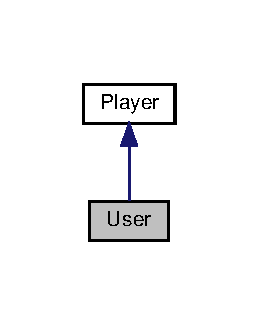
\includegraphics[width=124pt]{classUser__inherit__graph}
\end{center}
\end{figure}


Collaboration diagram for User\+:
\nopagebreak
\begin{figure}[H]
\begin{center}
\leavevmode
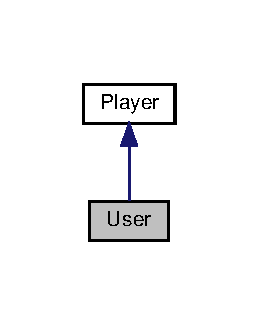
\includegraphics[width=124pt]{classUser__coll__graph}
\end{center}
\end{figure}
\subsection*{Public Member Functions}
\begin{DoxyCompactItemize}
\item 
void \hyperlink{classUser_acc17e3c44688c5f9f00f0a297ac4b7dc}{add\+Hit} (int x, int y)
\end{DoxyCompactItemize}


\subsection{Detailed Description}
This class inherits all \hyperlink{classPlayer}{Player} functionalities but is specified towards a user, not a bot. \begin{DoxyAuthor}{Author}
Adham Kassem 

Jonathon Henly 
\end{DoxyAuthor}


\subsection{Member Function Documentation}
\mbox{\Hypertarget{classUser_acc17e3c44688c5f9f00f0a297ac4b7dc}\label{classUser_acc17e3c44688c5f9f00f0a297ac4b7dc}} 
\index{User@{User}!add\+Hit@{add\+Hit}}
\index{add\+Hit@{add\+Hit}!User@{User}}
\subsubsection{\texorpdfstring{add\+Hit()}{addHit()}}
{\footnotesize\ttfamily void User\+::add\+Hit (\begin{DoxyParamCaption}\item[{int}]{x,  }\item[{int}]{y }\end{DoxyParamCaption})\hspace{0.3cm}{\ttfamily [inline]}}

This method is meant for user objects that represent the opponent user locally. When the server informs client that the clients turn was a hit, this method will change the local state of the grid for proper local visualization \begin{DoxyAuthor}{Author}
Adham Kassem 

Jonathon Henly 
\end{DoxyAuthor}

\begin{DoxyParams}{Parameters}
{\em x} & int \\
\hline
{\em y} & int \\
\hline
\end{DoxyParams}
\begin{DoxyReturn}{Returns}
none 
\end{DoxyReturn}


The documentation for this class was generated from the following file\+:\begin{DoxyCompactItemize}
\item 
include/User.\+h\end{DoxyCompactItemize}

%--- End generated contents ---

% Index
\backmatter
\newpage
\phantomsection
\clearemptydoublepage
\addcontentsline{toc}{chapter}{Index}
\printindex

\end{document}
